\documentclass[11pt]{article}
\usepackage{amsmath,amssymb,amsthm}
\usepackage{graphicx}
\usepackage[margin=1in]{geometry}
\usepackage{fancyhdr}
\usepackage{graphicx}
\usepackage{subcaption}
\setlength{\parindent}{0pt}
\setlength{\parskip}{5pt plus 1pt}
\setlength{\headheight}{13.6pt}
\newcommand\question[2]{\vspace{.25in}\hrule\textbf{#1: #2}\vspace{.5em}\hrule\vspace{.10in}}
\renewcommand\part[1]{\vspace{.10in}\textbf{#1}}
\pagestyle{fancyplain}
\lhead{\textbf{\NAME\ (\ANDREWID)}}
\chead{\textbf{HW\HWNUM}}
\rhead{\today}

\begin{document}\raggedright
	\newcommand\NAME{Muhammed Burak Bugrul}
	\newcommand\ANDREWID{150140015}
	\newcommand\HWNUM{2}
	\question{Q1}{Block Placement Problem}
	\part{a)} In CSP model, blocks are variables to bet matched with integer. These integers will be placing order of the blocks. While matching an integer to a block, requirements(supporting from center etc.) will be checked.\\
	\part{b)} After compiling blocks.cpp with command: "g++ blocks.cpp -std=c++14 -O2 -o blocks". Code can be run with command "./blocks 1 < {input file path} > {output file path}". 1 is for DFS algorithm. Code is written in C++ language. "center.txt, input.txt, input2.txt, input3.txt, input4.txt" are some example input files.\\
	\part{c)} Algorithm will not stuck, because there is a finite set of moves and there is visited control. If it can find a proper solution it returns it immediately.\\
	\part{d)} Visualization program is implemented in Python3 with using pygame. "pip3 install pygame" is pygame installagiton command. After installation it can be run via "python3 draw.py {output file path of c++ code}" command.
	
	\question{Q2}{Connect Four}
	\part{a)}
	\begin{figure}[h!]
		\centering
		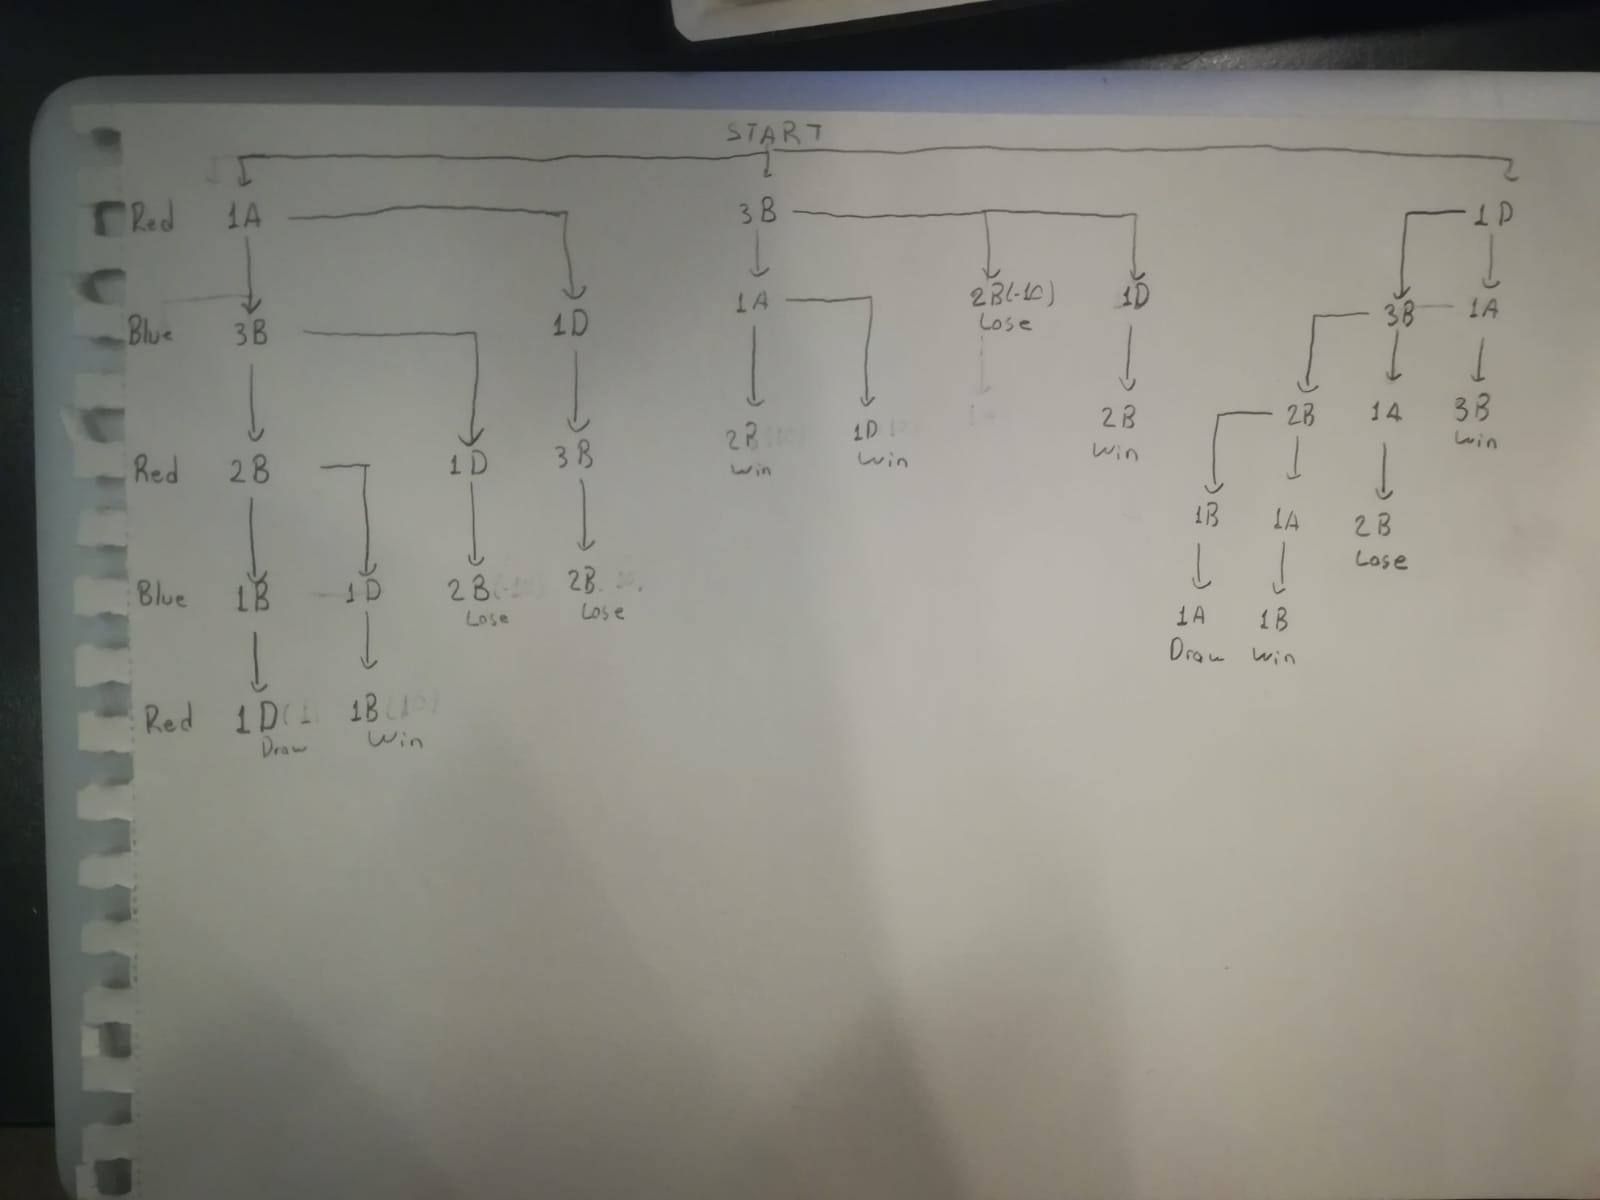
\includegraphics[width=0.5\textwidth]{tree.jpeg}
		\caption{Tree}
		\label{fig:Tree}
	\end{figure}
		Red can not wing against blue.
	\question{Q3}{Students}
	It can be implemented by using "Prologue" logical programming language.
\end{document}